%%%%% slides template
% Giovanni Ramirez (ramirez@ecfm.usac.edu.gt)
% 20200828
% Require: images/ecfmByN.png images/usacByN.jpg
%
%
% Use this option to print notes only
% \documentclass[xcolor=dvipsnames,handout,notes=only]{beamer}%
%
% Use this option to print notes and slides
% \documentclass[xcolor=dvipsnames,handout,notes=show]{beamer}%
%
% Use this option to get a printer-friendly version
% \documentclass[xcolor=dvipsnames,handout]{beamer}%
%
% Unse this option to get slides only
\documentclass[xcolor=dvipsnames,presentation]{beamer}%
%
%%%%%


%%%%% theme and coloring
% a list of themes can be found here https://hartwork.org/beamer-theme-matrix/
% I like a simple Malmoe with some modifications and color-schemes like
% dolphin for a white background, beetle for a gray background or dove for
% plain slides
%
% theme definition
\usetheme{Malmoe}
%
% definition of the presentation mode: full slides
\mode<presentation> {
% coloring for slides other options: beetle, dove
  \usecolortheme{dolphin}
% to include a slide with the table of contents
 \AtBeginSection[] {
  \begin{frame}
    \tableofcontents[currentsection]
  \end{frame} }
}
%
% definition of the handout mode: printer-friendly
\mode<handout>{
% coloring: dove is white
  \usecolortheme{dove}
% this is to print 2 slides in 1 page, other values are allowed
  \usepackage{pgfpages}
  \renewcommand\textbullet{\ensuremath{\bullet}}
  \pgfpagesuselayout{2 on 1}[letterpaper,border shrink=5mm]
% set the fontsize of the notes
  \setbeamerfont{note page}{size=\scriptsize}
% disable the slide with the table of contents
  \AtBeginSection[]{}
}
%%%%%

%%%%% personalisation
% clear all headers
\setbeamertemplate{headline}{}
% disable navigation buttons
\setbeamertemplate{navigation symbols}{}
% configure the blocks used for equations, theorems, etc
\setbeamertemplate{blocks}[rounded][shadow=true]
% clear the footline
\setbeamertemplate{footline}{}
% set the footline
\setbeamertemplate{footline}{
  \hbox{%
% left block with the shortname, it is set in the \author command
    \begin{beamercolorbox}[wd=.25\paperwidth,ht=2.25ex,dp=1ex,center]%
      {author in head/foot}%
      \usebeamerfont{author in head/foot}\insertshortauthor
    \end{beamercolorbox}%
% center block with the short title, it is set in the \title command
    \begin{beamercolorbox}[wd=.65\paperwidth,ht=2.25ex,dp=1ex,center]%
      {title in head/foot}%
      \usebeamerfont{title in head/foot}\insertshorttitle
    \end{beamercolorbox}%
% right block with the number of slides
    \begin{beamercolorbox}[wd=.10\paperwidth,ht=2.25ex,dp=1ex,right]%
      {date in head/foot}%
      \usebeamerfont{date in head/foot}
      \insertframenumber{} / \inserttotalframenumber\hspace*{1em}
    \end{beamercolorbox}}%
  \vskip0pt%
}
%%%%%

%%%%% packages
%
% language, decimal point mark
\usepackage[spanish,es-nodecimaldot]{babel}%
%
% to use only T1 scalable fonts
\usepackage[T1]{fontenc}%
\let\Tiny=\tiny% this is a proper configuration of the tiny font size
%
% to use UTF coding, other options latin1
\usepackage[utf8]{inputenc}%
%
\usepackage{array}
% special math symbols
\usepackage{latexsym,amsfonts,amsmath}%
%
% to include graphics
\usepackage{graphicx}%
% to include subfigures
\usepackage{subfigure}
% path to images
\graphicspath{{figs_avance/}}
%
% to use tiks: nice to draw diagrams
\usepackage{tikz}%
\usetikzlibrary{arrows,shapes,positioning}
%
% to use SI units and physics notation
\usepackage{physics}%
\usepackage{multirow}
\usepackage{xcolor}
%
% to use hypenation
\usepackage{ragged2e}%
\let\raggedright=\RaggedRight%
%
\usepackage{dsfont}

\usepackage[draft,inline,nomargin]{fixme} \fxsetup{theme=color}
\newcommand\dsone{\mathds{1}}
\definecolor{jacolor}{RGB}{200,40,0} \FXRegisterAuthor{ja}{aja}{\color{jacolor}JA}
% to configure the hyperref to set metadata in the PDF file
\hypersetup{%
%pdfpagemode=FullScreen,% to open the file in fullscreen
breaklinks={true},% to allow links in more than one line
%pdfstartview={Fit},% to set the slide to fit the screen
%pdfpagemode=FullScreen,% to set it to full screen
pdfauthor={Giovanni Ramirez Garcia (ramirez@ecfm.usac.edu.gt)},% author name
pdftitle={Quantum Optics aplied to Quantum Computing},% title of the talk
pdfsubject={Keynote for the talk at Lat0 group},% subject of the talk
pdfkeywords={quantum optics, quantum computing, quantum algorithms, quantum
  circuits}% keywords to categorise the contents
}
%%%%%

\newcommand{\shk}{Sherrington-Kirkpatrick}
\newcommand{\syr}{Šimkovic y Ross}

%%%%% Talk data
%
%title
\title[Avance proyecto]% this is the short title
{\bf Avance proyecto Método de Monte Carlo de cadenas de Markov 
de muchas configuraciones (MC${}^3$)}% this is the long title
%
% author
\author[J. A. de León]% this is the short name
{José Alfredo de León}% this is the long name
%
% affiliation
%\institute{${}^1$Escuela de Ciencias Físicas y Matemáticas, U. de 
%San Carlos de Guatemala\newline%
%${}^2$Instituto de Física, U. Nacional Autónoma de México\newline
%${}^3$Departamento de Física, U. Federal de Pernambuco}%
%
% date and information about the conference
\date{\today}
%%%%%


\begin{document}
% % % % % % % % % % % % % % % % % % % % % % % % % % % % % % % % % % % % % %
% Title and Outline
% % % % % % % % % % % % % % % % % % % % % % % % % % % % % % % % % % % % % %
\begin{frame}[plain]
%	\janote{figuritas de canales cuánticos}
  \titlepage %
%  \begin{tikzpicture}[x=1mm,y=1mm,overlay,remember picture]
%    \pgftransformshift{\pgfpointanchor{current page}{center}}
%    \node[inner sep=0pt] (usac) at (-35,-30) %
%    {\includegraphics[height=12mm]{logos/ecfmByN}};
%    \node[inner sep=0pt] (usac) at (0,-30) %
%    {\includegraphics[height=12mm]{logos/ifunam}};
%    \node[inner sep=0pt] (ecfm) at (35,-30) %
%    {\includegraphics[height=12mm]{logos/u-pernambuco}};
%  \end{tikzpicture}
\end{frame}

\begin{frame}{Contenido}
  \tableofcontents[hidesubsections] 
\end{frame}

{
\AtBeginSection{}
\section{Recordatorio del proyecto}
\begin{frame}{Recordatorio del proyecto}
El objetivo del proyecto es implementar el nuevo método de Monte Carlo
propuesto por \syr{} en \textcolor{Gray}{arxiv:2103.05613v1} en el cual
para cada paso Monte Carlo (MC) se explora una configuración de estados
y no un único estado. Específicamente, el proyecto consiste en reproducir
los resultados de \syr{} de su método aplicado para resolver los modelos
\begin{itemize}
\item \shk{}
\item Fermi-Hubbard
\end{itemize}
\end{frame}
}

{
\AtBeginSection{}
\section{Tareas realizadas}
\begin{frame}{Tareas realizadas}
\begin{itemize}
\item Estudiar el modelo de \shk{}.
\item Estudiar el método de Monte Carlo de cadena de Markov (MCMC).
\item Implementar en Mathematica el método MCMC para resolver 
el modelo de \shk{}.
\end{itemize}
\end{frame}
}

%\begin{frame}{Qué se ha hecho hasta ahora}
%Se implementó el método MCMC (algoritmo de Metrópolis- Hastings)
%para resolver el modelo de \shk{} y reproducir los resultados de la gráfica
%tal...
%
%Fallé... 
%\end{frame}

{
\AtBeginSection{}
\section{Modelo de \shk{}}
\begin{frame}{Modelo de \shk{}}
El modelo de \shk{} es un modelo propuesto en 1975 para modelar vidrios 
de espín. Es un modelo de Ising en el cual se consideran interacciones 
ferromagneticas y paramagnéticas de largo alcance. El Hamiltoninano 
del modelo está dado por 
\begin{align*}
\hat H=\frac{1}{\sqrt{L}}\sum_{j\leq k}J_{jk}\hat S_j\hat S_k,
\end{align*}
donde $L$ es el tamaño de la red, $J_{jk}$ son los parámetros de 
interacción y $\hat S_j$ los operadores de espín.

\begin{figure}

\includegraphics[width=2cm]{spin_glass}
%\caption{Figura esquemática del modelo de Sherrington-Kirkpatrick. Tomada de Wikipedia.}
%\label{fig:shk}
\end{figure}
\end{frame}
}

{
\AtBeginSection{}
\section{Algoritmo de Metrópolis-Hastings (MCMC)}
\begin{frame}{Algoritmo de Metrópolis-Hastings (MCMC)}
\begin{enumerate}
\item \textbf{Inicializar la configuración}.
\begin{enumerate}
\item Generar una configuración aleatoria de $L$ espines\\
$\{ \uparrow,\downarrow,\downarrow,\uparrow,\ldots,\uparrow\}$.
\item Generar los parámetros de interacción reales $J_{jk}$ con números que 
obedecen una PDF Gaussiana con media 0 y desviación igual a 1.
\item Calcular la energía inicial de la configuración\\
$E_0=1/\sqrt{L}\sum_{j\leq k}J_{jk}S_jS_k$.
%, siguiendo
%la expresión en \eqref{eq:SK:H}.
\item Elegir aleatoriamente un sitio $s$ para ``voltear'' al espín en 
ese sitio ($\uparrow\ \to\ \downarrow$ o $\downarrow\ \to\ \uparrow$).
\end{enumerate}
\item \textbf{Pasos Monte Carlo}. 
\begin{enumerate}
\item Calcular la energía $E_f$ de la nueva configuración con el espín en el
sitio $s$ invertido.
\item Si $E_f<E_0$, la nueva configuración es aceptada. Si $E_f>E_0$,
entonces la nueva configuración se acepta con una probabilidad 
$P_{\text{aceptación}}=e^{-(E_f-E_0)/k_BT}$ ($k_B=1$).
\item Escoger un nuevo sitio según una PDF Gaussiana con media
igual al sitio anterior y desviación estándar igual a $3$.
Para este paso, se deberán considerar condiciones periódicas.
\end{enumerate}
\end{enumerate}
\end{frame}
}

{
\AtBeginSection{}
\section{Resultados}
\begin{frame}{Resultados}
Se implementó el método MCMC para resolver el modelo de \shk{} con
una red de tamaño $L=10^3$ y a $T=1$.
\begin{figure}
\centering
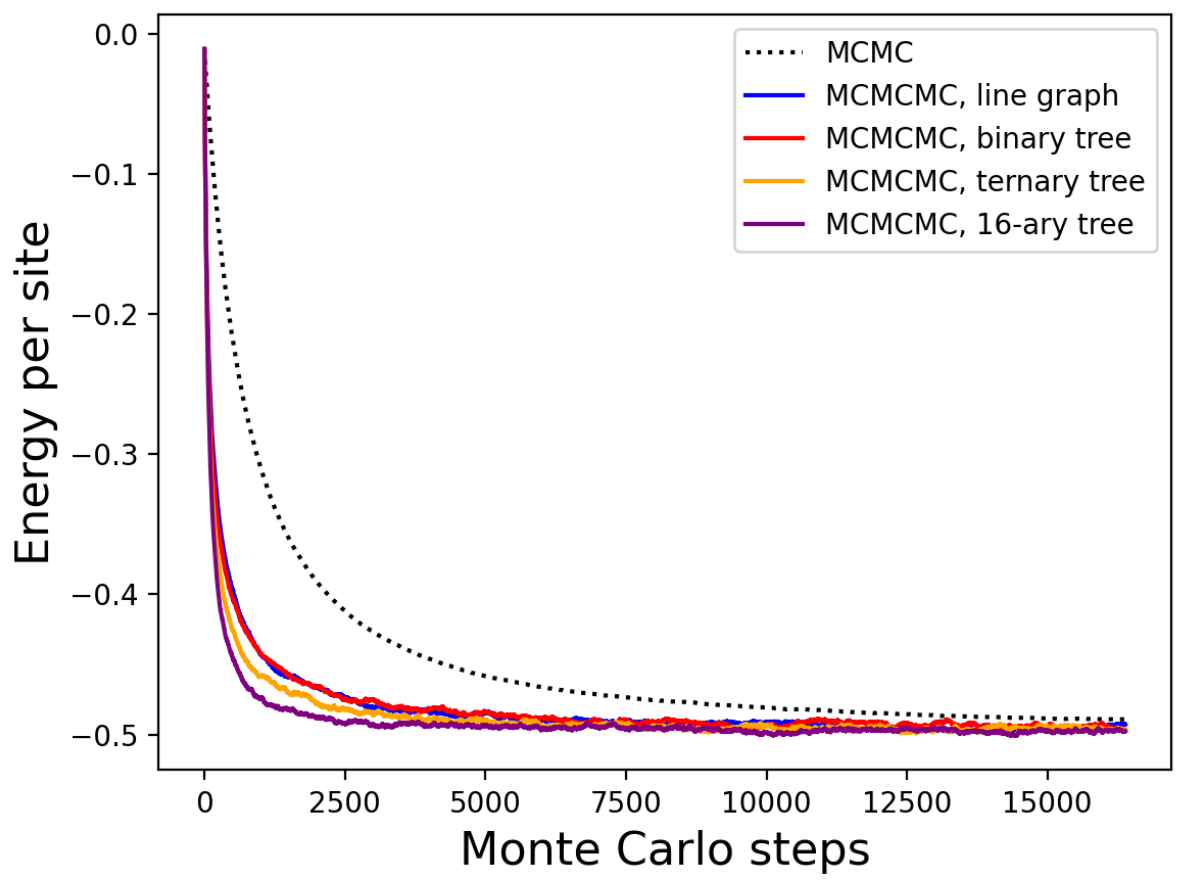
\includegraphics[width=8cm]{resultados}
\end{figure}
\end{frame}

\begin{frame}{Resultados}
\begin{figure}
\centering
\subfigure[]{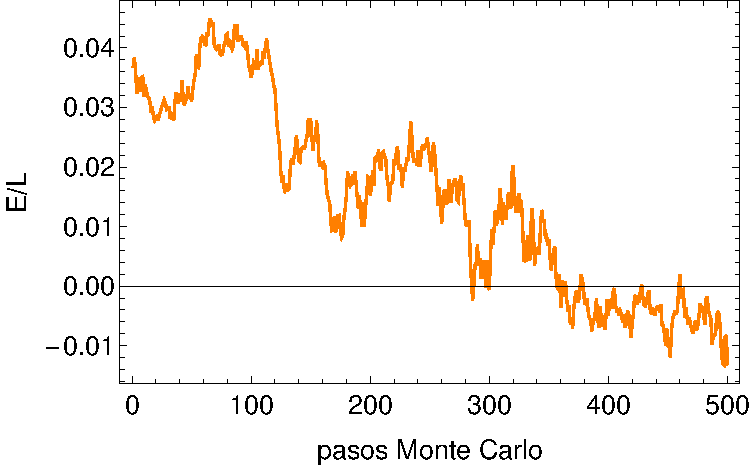
\includegraphics[height=2.9cm]{intento_001}}
\subfigure[]{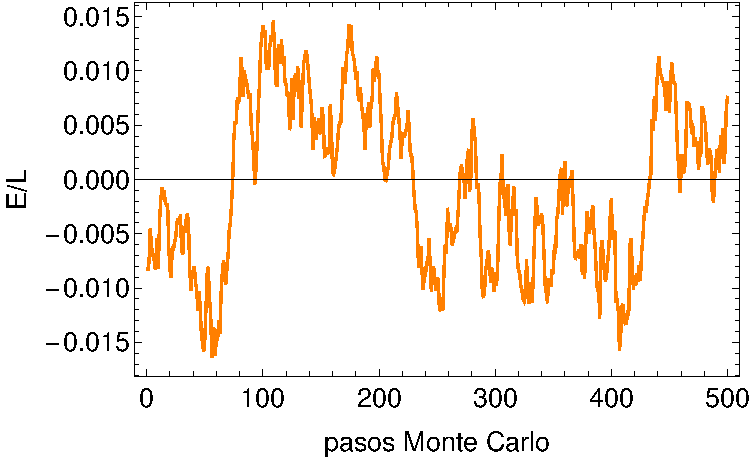
\includegraphics[height=2.9cm]{intento_002}}
\subfigure[]{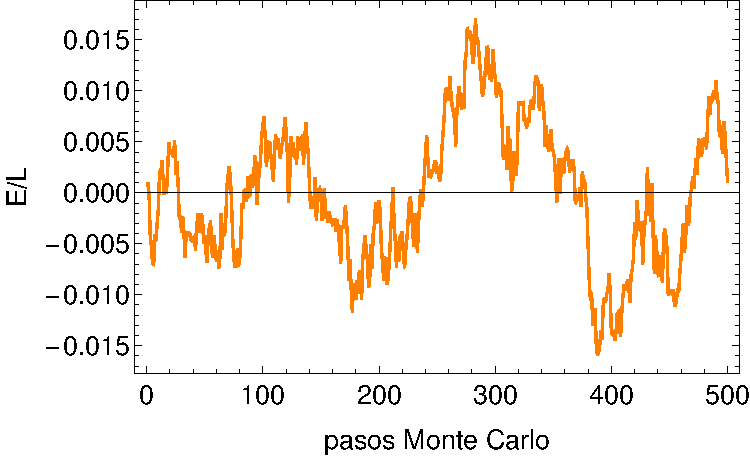
\includegraphics[height=2.9cm]{intento_003}}
\subfigure[]{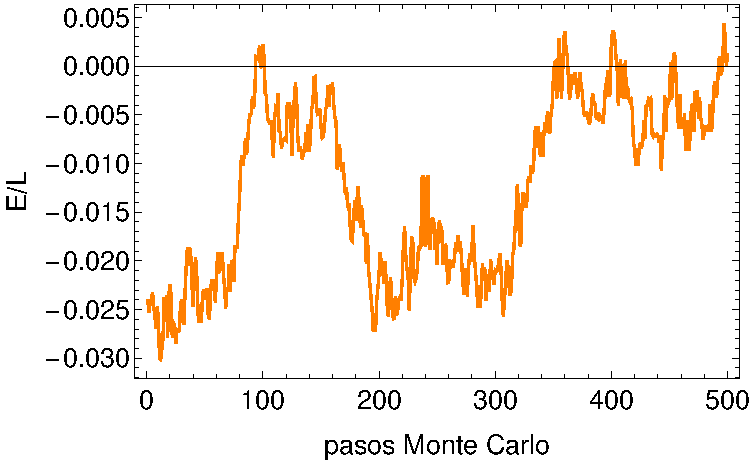
\includegraphics[height=2.9cm]{intento_004}}
\caption{PDF constante para escoger sitio en la nueva configuración.}
\end{figure}
\end{frame}
}

\begin{frame}{Hipótesis sobre los errores}
\begin{itemize}
\item La función de distribución de probabilidad que obedece 
la forma de elegir un nuevo sitio en la red está incorrecto. 
\item La probabilidad de aceptación $P_{\text{aceptación}}$ de una nueva
configuración de espines cuando esta aumenta la energía está chueca
(acepta demasiados pasos que aumentan la energía).
\item En la configuración inicial se escogen desproporcionadamente 
más espines en una dirección que en otra.
\end{itemize}
\end{frame}

\begin{frame}
\begin{figure}
\centering
\subfigure[$\sigma=2$]{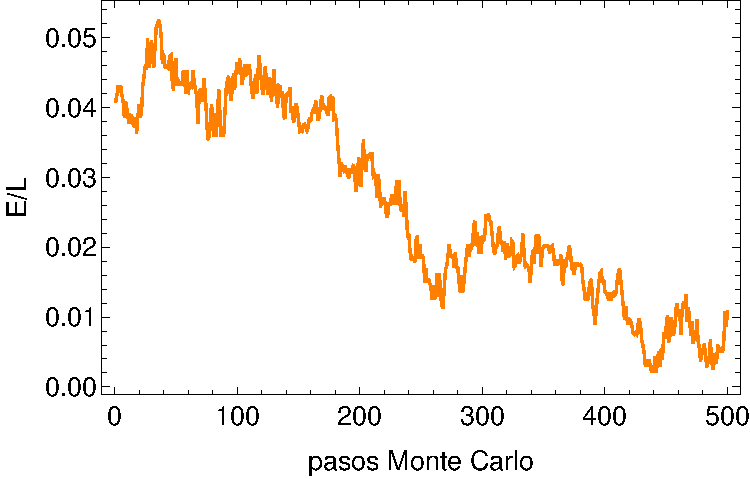
\includegraphics[height=3cm]{intento_005}}
\subfigure[$\sigma=5$]{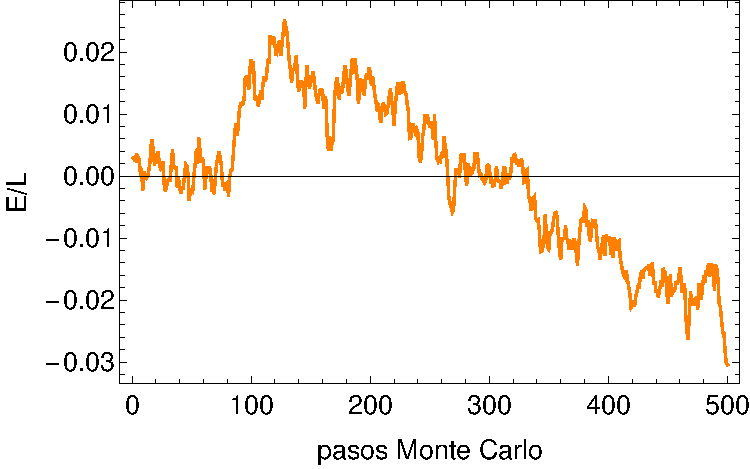
\includegraphics[height=3cm]{intento_006}}
\subfigure[$\sigma=10$]{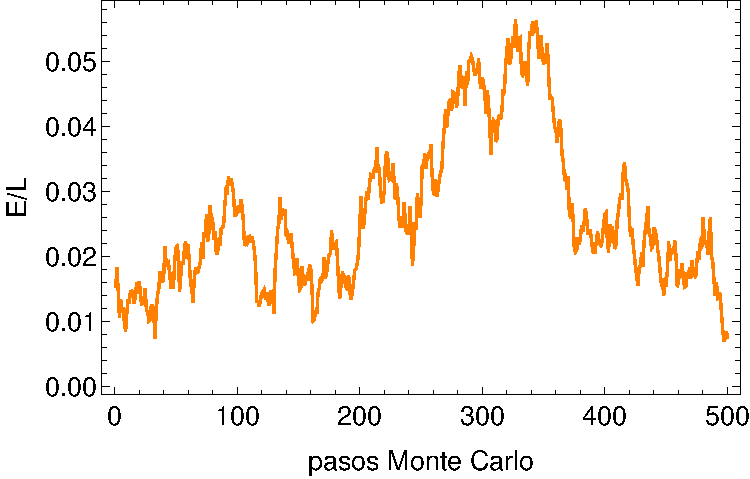
\includegraphics[height=3cm]{intento_007}}
\subfigure[$\sigma=50$]{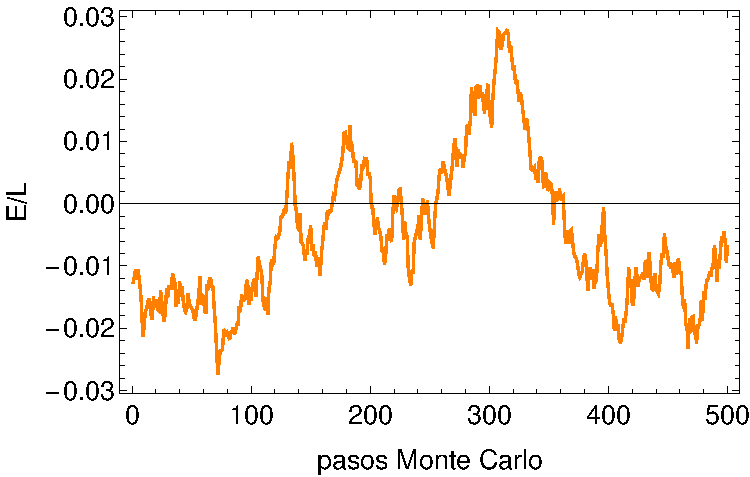
\includegraphics[height=3cm]{intento_008}}
\caption{PDF Gaussiana para escoger sitio en la nueva configuración.}
\end{figure}
\end{frame}

\begin{frame}
\begin{figure}
\centering
%\subfigure[]{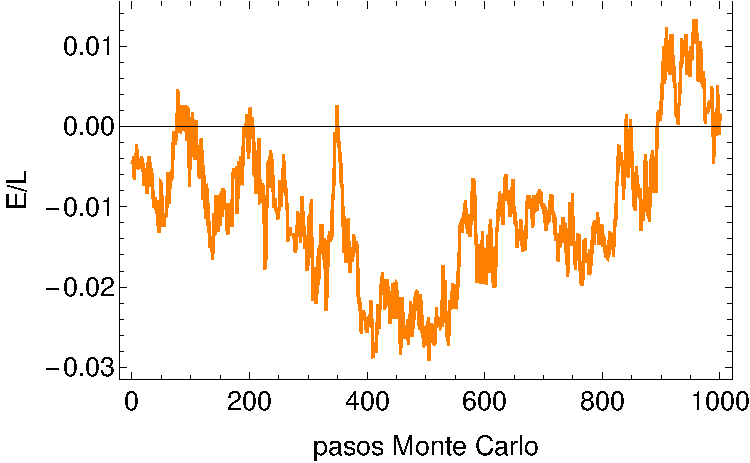
\includegraphics[height=3cm]{intento_009}}
\subfigure[$P_{\text{aceptación}}=1/3$]{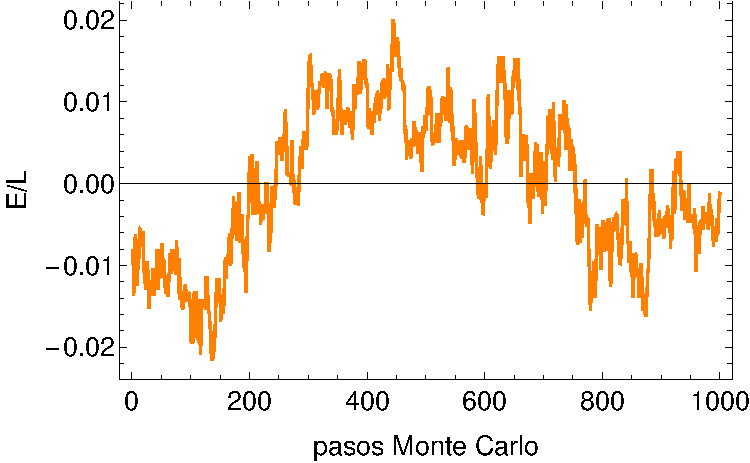
\includegraphics[height=3cm]{intento_012}}
\subfigure[$P_{\text{aceptación}}=1/4$]{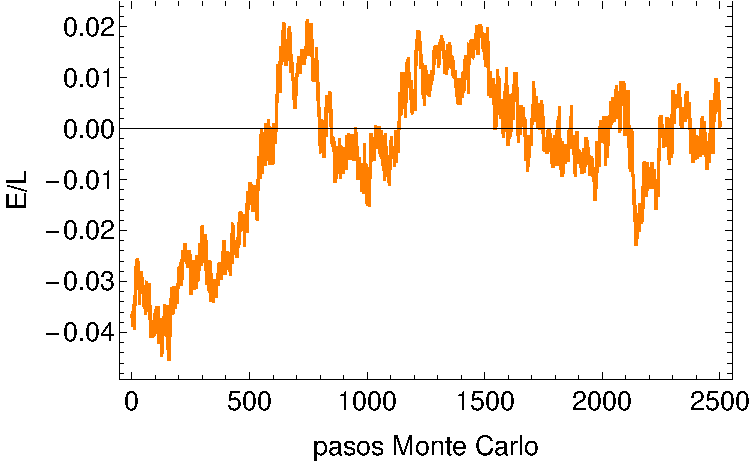
\includegraphics[height=3cm]{intento_013}}
\subfigure[$P_{\text{aceptación}}=1/5$]{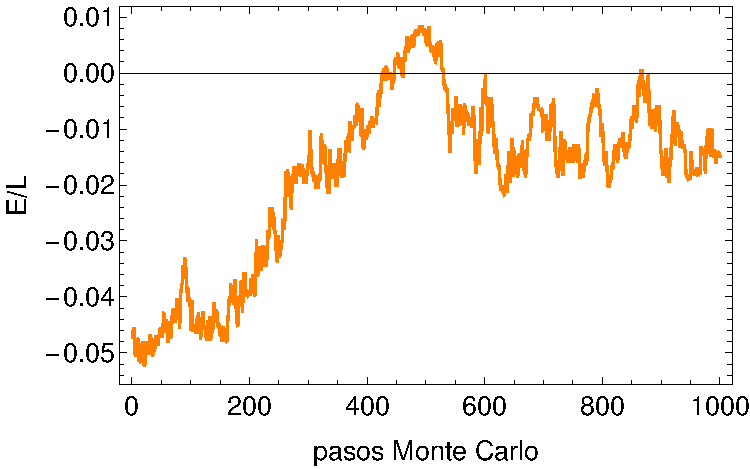
\includegraphics[height=3cm]{intento_014}}
\caption{Energía por sitio en función de pasos MC. PDF constante
 para escoger sitio en la nueva configuración.}
\end{figure}
\end{frame}

{
\AtBeginSection{}
\section{Conclusiones}
\begin{frame}{Conclusiones}
\begin{itemize}
\item No hay evidencia para decir si tomar una PDF constante o Gaussiana 
es mejor para escoger el nuevo sitio.
\item No hay evidencia para sostener la hipótesis de que la \\
$P_{\text{aceptación}}=e^{-(E_f-E_0)}$ sea la culpable de los resultados.
\item Se revisó que para la configuración inicial se utilice una 
PDF constante para escoger los espines en ambas direcciones.
\end{itemize}
\end{frame}
}

{
\AtBeginSection{}
\section{De última hora}
\begin{frame}{De última hora}
\begin{figure}
\centering
%\subfigure[]{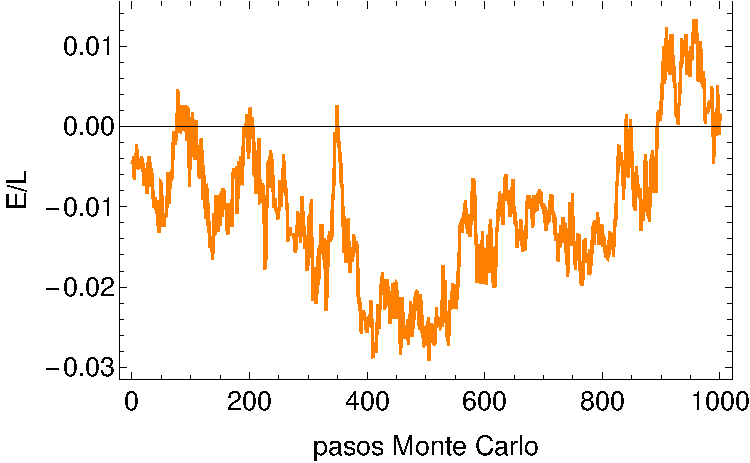
\includegraphics[height=3cm]{intento_009}}
\subfigure[]{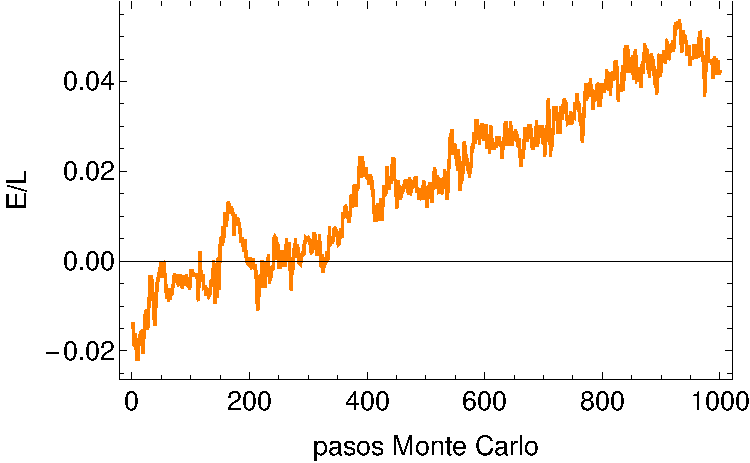
\includegraphics[height=3cm]{intento_101}}
\subfigure[]{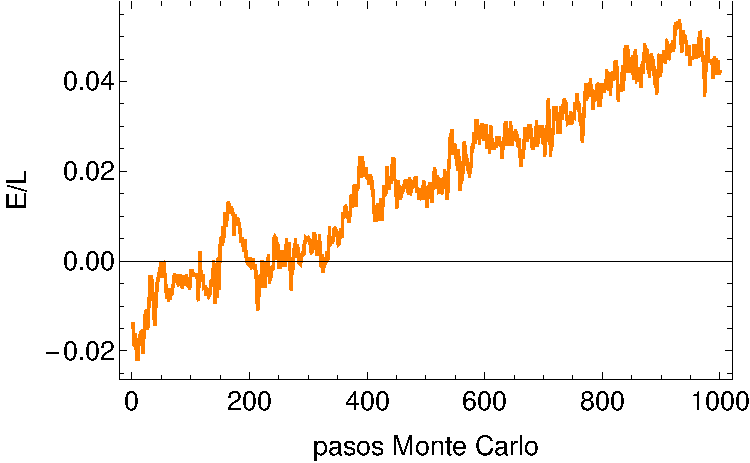
\includegraphics[height=3cm]{intento_101}}
\caption{El código está chueco. Método 
MCMC con $P_{\text{aceptación}}=0$.}
\end{figure}
\end{frame}
}

\end{document}

%%% Local Variables:
%%% mode: latex
%%% TeX-master: t
%%% End:
